\documentclass[12pt]{article}
\usepackage[margin={0.1in,0.1in}]{geometry}
\usepackage{multicol}
\usepackage{fullpage}
\usepackage{times}
\usepackage[normalem]{ulem}
\usepackage{multirow}
\usepackage{fancyhdr,graphicx,amsmath,amssymb, mathtools, scrextend, titlesec, enumitem}\usepackage[pdftex]{hyperref}
\usepackage[ruled,vlined]{algorithm2e}
\usepackage{parskip}
\usepackage{listings}
\usepackage{amsmath}
\usepackage{physics}
\usepackage{bbm}
\usepackage{titling}
\usepackage{bm}
\usepackage{geometry}
\geometry{top=1cm, left=1cm, bottom=1.5cm, right=1.5cm, margin=1cm}
\newcommand{\varvec}[2][n]{#2_1,\ldots, #2_#1}
\newcommand{\Var}{\mathrm{Var}}
\newcommand{\Bias}{\mathrm{Bias}}
\newcommand{\Cov}{\mathrm{Cov}}
\newcommand{\E}{{\rm I\kern-.3em E}}
\newcommand{\Binomial}{\mathrm{Binomial}}
\newcommand{\Bernoulli}{\mathrm{Bernoulli}}
\newcommand{\Poisson}{\mathrm{Poisson}}
\newcommand{\Normal}{\mathcal{N}}
\newcommand{\one}{\mathbbm{1}}
\newcommand{\Beta}{\text{Beta}}
\newcommand{\BetaPDF}{\text{Beta}}
\newcommand{\GammaPDF}{\text{Gamma}}
\newcommand{\Uniform}{\mathrm{Uniform}}
\newcommand{\QED}{\newline \mbox{} \hfill $\blacksquare$}
\newcommand{\Real}{\mathbb{R}}
\newcommand{\Sgn}{\mbox{Sgn}}
\renewcommand*{\arraystretch}{1.4}
\newtheorem{theorem}{Result}
\newtheorem{definition}{Definition}
\lstset{frame=tb,
	language=Python,
	aboveskip=3mm,
	belowskip=3mm,
	showstringspaces=false,
	columns=flexible,
	basicstyle={\small\ttfamily},
	numbers=none,
	stringstyle=\color{mauve},
	breaklines=true,
	breakatwhitespace=true,
	tabsize=3
}
\title{Computation Theory Note}
\usepackage{tikz}
\usetikzlibrary{automata, positioning, arrows}
\author{Ran Xie}

\begin{document}
	\maketitle
\section{Regular Languages}

% { \epsilon }
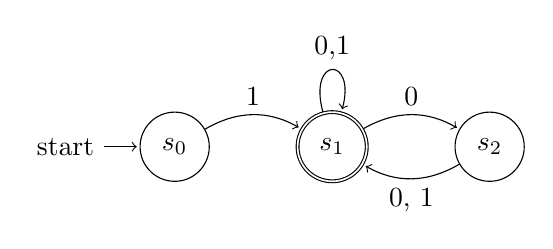
\begin{tikzpicture}[shorten >=1pt,node distance=2cm,on grid,auto]
	
	\node[state,initial]  (s_0)     {$s_0$};
	\node[state,accepting] (s_1) [right of=s_0]    {$s_1$};
	\node[state]  (s_2) [right of=s_1]  {$s_2$};
	
	\path[->]
	(s_0) edge [bend left]     node {1}  (s_1)
	(s_1) edge [loop above]  node {0,1}  ()
	      edge [bend left] node {0} (s_2)
	(s_2) edge [bend left] node {0, 1} (s_1);
\end{tikzpicture}

\textbf{state diagram} of \textbf{finite automaton} $M$. $q_0,q_1,q_2$ are \textbf{states}. $q_0$ is \textbf{start state}. $q_1$ is \textbf{accept state}. Arrows are called \textbf{transitions}. Input is string of 0s and 1s. The output is either \textbf{reject} or \textbf{accept}.\\

\textbf{(Deterministic) Finite Automaton (DFA)} $M$ is 5-tuple $(Q, \Sigma, \delta, q_0, F)$ where
\begin{enumerate}
	\item $Q$ is a finite set called the states
	\item $\Sigma$ is a finite set called the alphabet
	\item $\delta : Q \times \Sigma \rightarrow Q$ is the transition function
	\item $q_0 \in Q$ is the start state
	\item $F \subseteq Q$ is the set of accept states.
\end{enumerate}

\textbf{Language of machine }$M$, $A$ is the set of all strings that $M$ accepts and write $L(M) = A$. We say $M$ accepts $A$ or $M$ recognizes $A$. \\

\textbf{Language operations}: Let $A$ and $B$ be languages 
\begin{enumerate}
	\item Union: $A\cup B = \{x|x\in A \mbox{ or } x\in B\}$
	\item Concatenation: $A \circ B = \{xy| x\in A, y\in B\}$
	\item Star: $A^* = \{x_1x_2\ldots x_k| k \geq 0 \mbox{ and } x_i \in A \}$
\end{enumerate}

\textbf{Regular Language} is a language accepted by some finite automatons. The class of regular language is closed under union, concatenation and star operation. \\

\textbf{Nondeterministic finite automaton (NFA)} is 5-tuple $(Q,\Sigma,\delta,q_0, F)$.
\begin{enumerate}
	\item $Q$ is finite set of states
	\item $\Sigma$ is finite alphabet
	\item $\delta: Q\times \Sigma_\epsilon \longrightarrow P(Q)$
	\item $q_0\in Q$ is the start state
	\item $F \subseteq Q$ is the set of accept states
\end{enumerate}
\textbf{Remark}: $\epsilon$ is empty string. The transition function maps current input or $\epsilon$ and the current state to produce a set of next states (in the power set $P(Q)$) rather than a single next state in DFA. NFA accepts $w = y_1y_2\ldots y_m$ if $y_i \in \Sigma_\epsilon$ for all $i$ and a sequence of states $r_0, \ldots, r_m \in Q$ exists such that \begin{itemize}
	\item $r_0 = q_0$
	\item $r_{i+1} \in \delta (r_i, y_{i+1})$ for $i = 0, \ldots, m-1$
	\item $r_m \in F$
\end{itemize}
This means even NFA branches out but if one sequence of states exists such that the last state is in $F$, the NFA accepts the input.\\

\begin{theorem}
	Two automatons are equivalent if they recognizes the same language. Every NFA has an equivalent DFA. It follows that a language is regular if some NFA recognizes it.
\end{theorem}

$R$ is \textbf{Regular Expression} if $R$ is \begin{enumerate}
	\item $a$ for some $a$ in the alphabet $\Sigma$
	\item $\epsilon$
	\item $\emptyset$
	\item $(R_1 \cup R_2)$  (Union)
	\item $(R_1 \circ R_2)$ (Concatenation)
	\item $(R_1^*)$ (Star)
\end{enumerate}
where $R_1$ and $R_2$ are regular expressions. This type of definition is called \textbf{Inductive definition} (not a circular one).

\begin{theorem}
	A language is regular iff some regular expression describes it.
\end{theorem}

A \textbf{Generalized nondeterministic finite automaton (GNFA)} is a 5-tuple $(Q, \Sigma, \delta, q_{\text{start}}, q_{\text{accept}})$ where \begin{enumerate}
	\item $Q$ is the finite set of states
	\item $\Sigma$ is the input alphabet
	\item $\delta: (Q - \{q_{\text{start}}\}) \times (Q - {\text{accept}}) \longrightarrow R$ is the transition function.
	\item $q_{\text{start}}$ is the start state and $q_{\text{accept}}$ is the accept state.
\end{enumerate}

\section{Context Free Grammar}
Finite automata and regular expressions are methods to describe languages. Context-Free grammar is a more powerful method of describing languages. Languages described as called Context Free Languages.

A \textbf{grammar} consists of a collection of substitution rules also called \textbf{productions}. E.g.:
$$
\begin{aligned}
	&A \rightarrow 0A1 \\
	&A \rightarrow B \\
	&B \rightarrow \# \\
\end{aligned}
$$
$\{A, B\}$ are variable symbols. $\{0, 1, \# \}$ are terminal symbols. $A$ is the start variable. We say $A$ yields $0A1$ written $A \Rightarrow 0A1$. $A$ derives $0\#1$ written $A \stackrel{*}{\Rightarrow} 0\#1$ because there exists $A \Rightarrow 0A1 \Rightarrow 0B1 \Rightarrow 0\#1$

Formally, A \textbf{Context Free Grammar} is a 4-tuple $(V, \Sigma, R, S)$ where
\begin{enumerate}
	\item $V$ is a finite set called the variables
	\item $\Sigma$ is a finite set, disjoint from $V$ called the terminals
	\item  $R$ is a finite set of rules, with each rule being a variable and a string of variables and terminals
	\item $S \in V$ is the start variable.
\end{enumerate}

\end{document}